\chapter{Realisierung}
\minitoc
In diesem Kapitel wird die Realisierung des Entwicklungssystems
beschrieben. <\ldots>
\section{Konfiguration des Carambola}\label{sec:conf}
OpenWRT bietet mit dem Programm \gls{uci} eine Anwendung, Einstellungen
zentralisiert zu verwalten. Über das \gls{uci}-System lassen sich unter anderem
Ethernet, WLAN, DHCP und SSH-Server konfigurieren. Die einzelnen
Einstellungsdateien liegen alle im Verzeichnis \listinlsh{/etc/config/} und
können mittels des Tools modifiziert werden.

Nach Systemstart werden außerdem alle Dateien im Ordner
\listinlsh{/etc/uci-defaults/} eingelesen, ausgeführt und anschließend gelöscht.
Dies erlaubt es Softwarepaketen, Einstellungen am System vorzunehmen. Werden
diese Softwarepakete bereits in die Firmware integriert, entspricht dies einer
Art Vorkonfiguration des Systems.

Da alle diese Einstellungen für das zu entwerfende Entwicklungssystem spezifisch
sind, wird diese Datei zusammen mit der kompilierten Serveranwendung installiert
und nach einem Neustart beziehungsweise einem ersten Systemstart ausgeführt.
\subsection{WLAN und Netzwerkkonfiguration}
Da die Netzwerkkonfiguration von OpenWRT vollständig durch die
\gls{uci}-Konfigurationsdateien abgewickelt wird, muss auch \gls{uci} genutzt
werden, wenn das Netzwerk vorkonfiguriert werden soll.

\gls{uci} bietet mit \listinlsh{uci batch} explizit einen Befehl an, um
umfangreiche Einstellungsändeurngen vorzunehmen. Hierfür werden die einzelnen
Befehle mittels \emph{Here document} übergeben.
\begin{lstlisting}[language=sh]
uci batch <<-EOF_network
	...
	commit network
	EOF_network
\end{lstlisting}
\begin{definition}[Here document]
Ein \emph{Here document} ermöglicht es, einem Unix-Befehl mehrere, durch
Zeilenumbrüche getrennte, Befehle zu übergeben.
\end{definition}
Da diese Einstellungen nur einmalig getätigt werden müssen, wird dafür die in
\autoref{sec:conf} erwähnte Datei in \listinlsh{/etc/uci-defaults/} verwendet.

\subsection{Aktivierung des UART}\label{subs:aktuart}
Der Mikrochip\cite{RA01} des Carambolas besitzt zwei \glspl{uart}. Einer dieser
\glspl{uart} wird für die Serielle Konsole verwendet und somit kann der zweite
Anschluss für die Datenschnittstelle des Entwicklungssystems verwendet werden.
Da die Pins des Carambolas für den zweiten \gls{uart} standardmäßig auf
\gls{gpio}-Betrieb eingestellt sind, müssen diese erst umgestellt werden.

Hierzu muss das Tool \texttt{io} installiert und mittels 
\listinlsh{io 0x10000060 0x01} ausgeführt werden. Dies setzt im Speicher des
Mikrocontrollers das Flag, den \gls{uart} zu aktivieren. Dieser Vorgang muss
nach jedem Systemstart erfolgen und kann durch die, bei jedem Systemstart
aufgerufene, \listinlsh{/etc/rc.local} erfolgen.

Zusätzlich muss verhindert werden, dass auf diesem \gls{uart} eine Linuxterminal
betrieben wird. Hierzu muss die Datei \listinlsh{/etc/inittab} modifiziert
werden.

Diese beiden Änderungen werden wie folgt ebenso mittels des Skripts in
\listinlsh{/etc/uci-defaults/} nach \autoref{sec:conf} durchgeführt.
\begin{lstlisting}[language=sh]
sed -i '/exit 0/ i\io 0x10000060 0x01' /etc/rc.local
sed -i '/ttyS0/ s/^/# /' /etc/inittab
\end{lstlisting}

\section{OpenOCD}
Für OpenOCD existiert keine Portierung in die Paketverwaltung von OpenWRT. Es
muss also ein Makefile erstellt werden, das die Einbindung ermöglicht. Der
grundlegende Aufbau solcher Makefiles ist im Wiki von OpenWRT
festgelegt\cite{OWRT}.

Um OpenOCD kompilieren zu können, müssen zuerst die Voraussetzungen festgestellt
werden. Da ein auf dem FT2232-Chip basierender \gls{jtag}-Adapter mit
USB-Anschluss eingesetzt werden soll, müssen laut \texttt{README} von OpenOCD
sowohl libftdi als auch libusb installiert sein. Diese Pakete stehen für OpenWRT
bereits zur Verfügung und müssen im Makefile als Abhängigkeiten definiert
werden. Dies geschieht mit dem Befehl \listinlsh{DEPENDS:=+libftdi +libusb}.

Der Quellcode von OpenOCD in der Version 0.6.1 wird durch das Makefile von
Sourceforge selbstständig heruntergeladen, über MD5 verifiziert und entpackt.

Um eine hohe Kompatibilität gegenüber allen möglichen Zielsystemen zu
gewährleisten, musste das \texttt{Makefile} der \texttt{libftdi} angepasst werden, da die in den
Repositories vorhandene Version 0.19  keine Kommunikation mit Adaptern
gewährleistet, die einen FT232H-Chip besitzen. Diese Funktion gewährleistet erst
Version 0.20.

Vor dem Kompilierungsvorgang müssen noch die an \listinlsh{./configure}
zu übergebenden Argumente festgelegt werden. Der verwendete Adapter
verwendet einen FT2232H-Chip und erfordert daher die Option
\listinlsh{--enable-ft2232_libftdi}.
Die Option \listinlsh{--enable-parport} wird in der \texttt{README} von OpenOCD als
empfohlen angegeben und aktiviert die Unterstützung für \gls{jtag}-Adapter, die
den Parallelport verwenden.

\begin{lstlisting}[language=make]
CONFIGURE_ARGS+= \
	--prefix=$(STAGING_DIR)/usr \
	--enable-dummy \
	--enable-parport \
	--enable-ft2232_libftdi
\end{lstlisting}

Zu den Kompilerargumenten muss die Option
\texttt{-Wno-error=maybe-uninitialized} hinzugefügt werden, da anderenfalls
eine den Kompiliervorgang abbrechende Warnung beim Kompilieren der Datei
\texttt{src/target/dsp5680xx.c} auftritt.

\section{Server - FreeJTAG}
Der "`FreeJTAG"' genannte Server des Entwicklungssystems wird auf dem Carambola
installiert, als Serveranwendung bei jedem Systemstart gestartet und leitet die
gesammelten Daten an jeden verbundenen Client weiter.


\subsection{Bibliotheken und Abhängigkeiten}
Als Bibliotheken kommen bei FreeJTAG vor allem Teile der Boost Bibliothek zum
Einsatz. Diese dienen der asynchronen Netzwerkkommunikation (Boost ASIO), dem
hierfür nötigen Einsatz von Threads (Boost Thread), der Verwaltung der
Zeitstempel (Boost Chrono) und dem Speichern von Programmeinstellungen (Boost
Program\_Options).

Außerdem hängt FreeJTAG von dem Paket "`io"' ab, da dieses für die Aktivierung
des \gls{uart}, wie in \autoref{subs:aktuart} beschrieben, zuständig ist und
installiert werden muss. Die in \autoref{subs:aktuart} beschriebene Skriptdatei
ist ebenso in diesem Paket enthalten. 

Durch die Installation dieser Anwendung wird das Carambola also komplett für den
Einsatz als Entwicklungssystem konfiguriert.

\subsection{Strukturierung der Serversoftware}
\begin{figure}[!ht]
\centering
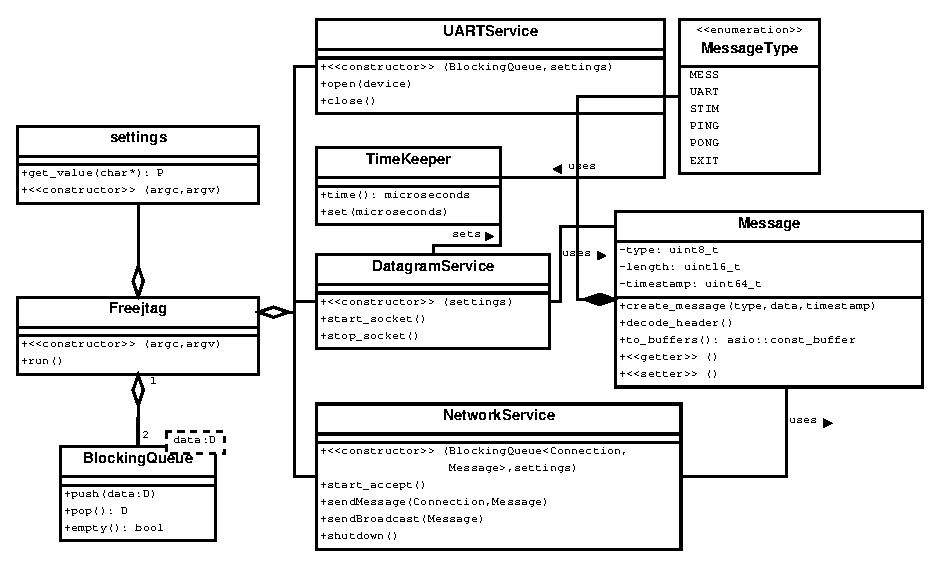
\includegraphics[width=\textwidth]{server.eps}
\caption{Grober Aufbau der Serveranwendung}{Diese Abbildung verdeutlicht den
Aufbau der Serveranwendung (FreeJTAG). Hierbei wurden Details zu Gunsten der
Übersichtlichkeit ausgelassen.}
\label{fig:server}
\end{figure}
\autoref{fig:server} stellt eine grobe Übersicht über den Aufbau der
Serveranwendung dar. Hierbei wurden Details wie weitere Klassen und
zusätzliche Aggregationen zwischen den einzelnen Elementen zugunsten einer
besseren Übersicht ausgelassen.

Die Hauptanwendung \texttt{Freejtag} dient als "`Bindeglied"' zwischen den
einzelnen Bestandteilen der Software. Die genaueren Abläufe hierzu sollen in
\autoref{subs:abl} erläutert werden.

Weiterhin besteht die Serversoftware aus einer Klasse
\texttt{NetworkService} zur Übertragung der Nutzdaten, \texttt{DatagramService}
um die Zeitsynchronisation über UDP zu managen und \texttt{UARTService} für den
Empfang der Daten vom Zielsystem.

Die Klasse \texttt{Message} dient zum Parsen der Netzwerkdaten und wird somit
sowohl vom TCP- als auch vom UDP-Dienst verwendet.

Da die Zeitstempel synchronisiert werden sollen, wurde die Klasse
\texttt{TimeKeeper} erstellt. Sie dient dem Setzen der Zeitdifferenz und der
Abfrage des aktuellen Zeitstempels unter Berücksichtigung der gespeicherten
Differenz.

Die Hilfsklasse \texttt{BlockingQueue} wird als Schnittstelle zwischen dem
Hauptprogramm und dem \texttt{UARTService} sowie zwischen dem Hauptprogramm
und dem \texttt{NetworkService} eingesetzt. Sie ist nötig, da jeder dieser
Dienste in einem anderen Thread läuft und der Datenaustausch aus diesem Grund
synchronisiert werden muss.

\subsection{Funktionsweise der Serversoftware}
In diesem Abschnitt sollen die wichtigsten Abläufe in der Serveranwendung
erläutert werden. Der Schwerpunkt liegt hierbei hauptsächlich auf der
Synchronisierung der Zeit und dem Weiterleiten der gesammelten Daten.
\subsubsection*{Programmstart}\label{subs:start}
Die Anwendung wird zuerst initialisiert und anschließend ausgeführt. Dies
erfolgt durch folgenden Ablauf.
\begin{lstlisting}[language=C++]
int main(int argc, char* argv[]) {
    freejtag::Freejtag *prog;
    prog = new freejtag::Freejtag(argc, argv);
    int res = prog->run();
    delete prog;
    return res;
}
\end{lstlisting}

Für die Funktion dieser Software müssen zu Beginn einige Einstellungen
festgelegt werden. Hierzu zählen die Parameter der \gls{uart}-Verbindung
(Baudrate, Parität, Stopp-Bit) und der Netzwerkport.

Bei Erstellung des \texttt{Freejtag}-Objektes werden zuerst die Werte aus
\listinlsh{/etc/freejtag.cfg} und die per Parameter (und in diesem Fall
Kommandozeile) übergebenen Argumente als Einstellungen eingelesen.
Das Einlesen dieser Werte erfolgt unter Nutzung der
\emph{Boost.Program\_options}-Bibliothek. Tritt hierbei ein Fehler auf, wird das
Programm mit einer Fehlermeldung beendet.

Intern werden die über das Netzwerk zu versendenden und empfangenen Nachrichten
mittels \listinlcpp{boost::shared\_ptr}(Smart Pointer) von
\texttt{Message}-Objekten verwendet. Es muss nun eine \\\texttt{BlockingQueue}
initialisiert werden, die die über den TCP-Port empfangenen Nachrichten
verwaltet. Da asynchrone TCP-Sendevorgängen mittels der
\listinlcpp{boost::asio}-Bibliothek erfolgen, ist eine weitere
\texttt{BlockingQueue} zur Synchronisierung hierfür nicht notwendig.

Da es möglich sein soll mehrere Verbindungen (Siehe auch \autoref{subs:best}) zu
verwalten, muss in der \texttt{BlockingQueue} zusammen mit der \texttt{Message}
auch immer die Verbindung von der sie erhalten wurde gespeichert werden.

Eine zweite \texttt{BlockingQueue} dient zur Erfassung der über UART gesammelten
Daten mit zugehörigen Zeitstempeln. 

Nun werden sowohl \texttt{NetworkService} als auch \texttt{DatagramService}
initialisiert.

Der \texttt{NetworkService} erhält hierfür die vorher erstellte
\texttt{BlockingQueue}(den Buffer), legt das Protokoll auf TCP fest und
öffnet den in den Einstellungen spezifizierten Port. Der Ablauf des
\texttt{DatagramService} verläuft analog mit dem Unterschied, dass für die über
diesen Dienst erfolgende Zeitsynchronisation kein Zugriff auf den
Nachrichten-Buffer nötig ist.

Anschließend werden zwei Threads gestartet, die für die Abwicklung der, durch
den Empfang von UART- oder Netzwerkdaten angestoßenen, Vorgänge zuständig
ist. Hierfür warten die Threads mittels \listinlcpp{UARTMessage msg =
input_uart_.pop();} beziehungsweise \newline\listinlcpp{MessageDatagram msgd =
input_network_.pop();} auf die Ankunft neuer Daten in ihrere zugehörigen
\texttt{BlockingQueue}. Dies schließt die Initialisierung ab.

Nun muss nun \listinlcpp{Freejtag::run();} aufgerufen werden, um den Start der
Anwendung zu vollziehen. Dies startet ein asynchrones Accept auf dem Socket des
Netzwerkmoduls, so dass es nun möglich ist, eine Verbindung zum Server
herzustellen. Der \gls{uart}-Anschluss wird auf dem angegebenen Gerät geöffnet
und mit den eingestellten Parametern konfiguriert.

Schließlich ruft der startende Thread die blockierende Methode
\listinlcpp{io_service_.run();} auf und dient nun zur Abarbeitung der
asynchronen Netzwerkvorgänge.
\subsubsection*{Zeitsynchronisation}\label{subs:servertime}
Die Synchronisation soll nach den Vorüberlegungen aus \autoref{subs:time}
erfolgen und auch die dort angegebenen Vorgaben einhalten.

Ein erster Ansatz wäre, bereits bestehende Synchronisationstechniken wie
\gls{ntp} zu verwenden. Diese haben jedoch den Nachteil, dass sie für die
Synchronisation immer eine aktive Verbindung zum Internet oder einen lokalen
NTP-Server  benötigen. Außerdem sind, da die Carambola-Systeme keine
Echtzeituhren besitzen, Datum und Uhrzeit nach einem Start des Systems auf die
Unix Epoche gesetzt. Da NTP direkt die Systemzeit beeinflusst, würde dies 
unter Umständen Auswirkungen auf andere Prozesse bedeuten.

Für die Zeitsynchronisation soll eine Abwandlung des Algorithmus von
Christian\cite{CHR} zum Einsatz kommen. Entscheidend ist hierbei, dass der
Synchronisationsvorgang vom Zeitgeber angestoßen wird. Dies erfordert eine
zusätzliche abschließende Datenübertragung.

Da TCP durch seine Flusskontrolle die Messung der Netzwerklatenz
durch eventuell Neuübertragungsversuche negativ beeinflussen kann, ist für die
Zeitsynchronisation die Verwendung von UDP nötig. Dies bedingt allerdings die
Verwendung einer Sequenznummer.

\begin{itemize}
  \item Der Client stößt den Synchronisationsvorgang an, indem er dem Server
  seinen aktuellen Zeitstempel $t_0$ mittels einer \texttt{PING}-Nachricht
  übermittelt.
  \item Bei Erhalt der Nachricht erfasst der Server seinen eigenen Zeitstempel
  als $t_1$.
  \item Anschließend bereitet er das Senden einer \texttt{PONG}-Nachricht als
  Antwort vor, erfasst einen weiteren Zeitstempel ($t_2$) und sendet die
  Nachricht.
  \item Bei Erhalt der Nachricht durch den Client, erfasst dieser seine eigene
  Zeit $t_3$ und übermittelt sie dem Server in einer, diesen
  Synchronisierungsprozess abschließenden, \texttt{STIM}-Nachricht.
\end{itemize} 
Dieser Vorgang ist in \autoref{fig:timeseq} visualisiert.

\begin{figure}
\centering
\begin{sequencediagram}[ht]
\newthread[0]{client}{:Client}
\newthread[3]{server}{:Server}
\mess[2]{client}{PING}{server}
\node[anchor=east,inner sep=10pt] (t0) at (mess from) {$t_0$};
\node[anchor=west,inner sep=4pt,label=above right:{$t_1$}] (t1) at (mess to)
{};
\mess[2]{server}{PONG}{client}
\node[anchor=west,inner sep=4pt,label=below right:{$t_2$}] (t2) at (mess from)
{}; \node[anchor=east,inner sep=10pt] (t3) at (mess to) {$t_3$};
\mess[2]{client}{STIM}{server}
\path (t0.east) |- coordinate(t01) (t1);
\draw[dashed] (t1) -- (t01);
\path (t3.east) |- coordinate(t23) (t2);
\draw[dashed] (t2) -- (t23);
\end{sequencediagram}
\caption{Ablauf der Zeitsynchronisation eines Servers}
\label{fig:timeseq}
\end{figure}

Nach Abschluss dieser Kommunikation lässt sich die Zeitdifferenz durch folgende
Formel errechnen.
\begin{equation}
\frac{t_1-t_0-t_3+t_2}{2}=\Delta t
\end{equation}
Um Abweichungen, zum Beispiel durch unterschiedliche Latenzen auf dem Hin- und
Rückweg im Netzwerk, auszugleichen, werden mehrere dieser Vorgänge durchgeführt
und ein arithmetisches Mittel über die gesammelten Differenzen gebildet. Dieser
Mittelwert ist eine etwas bessere Annäherung an die tatsächliche Differenz.

Da nun die Abweichung zur Clientsoftware ermittelt wurde, kann die Funktion
\newline\listinlcpp{TimeKeeper::set(microseconds difference)} verwendet werden,
um diesen Wert zu speichern. Durch diese Justierung wird der \texttt{TimeKeeper}
in diesem Augenblick effektiv auf \SI{0}{\micro\second} gesetzt.

Der aktuelle Zeitstempel wird bei Abfrage durch eine simple Subtraktion
errechnet.
\begin{lstlisting}[language=C++]
static high_resolution_clock::time_point epoch;
microseconds TimeKeeper::time(){
    high_resolution_clock::duration now = 
    			high_resolution_clock::now() - epoch;
    return duration_cast<microseconds>(now);
}
\end{lstlisting}

\subsubsection*{Empfang und Weiterleitung von UART-Daten}
Die Hauptfunktion des Servers liegt im Weiterleiten von über den
\gls{uart}-Anschluss erhaltenen Daten.

Ein beispielhafter Ablauf ist in \autoref{fig:serveruart} abgebildet.

Sobald die asynchrone Empfangsroutine des \texttt{UARTService} aufgerufen wird,
fragt diese den aktuellen Zeitstempel über den \texttt{TimeKeeper} ab. Zu
diesem Zweck besitzt dieser die statische Funktion \listinlcpp{time()}, die den
aktuellen Zeitpunkt in Mikrosekunden wie in \autoref{subs:servertime}
erläutert zurückgibt.

Anschließend wird der Zeitstempel zusammen mit der erhaltenen Textzeile in die
Buffer-Queue gegeben. Aus dieser Queue wird dieses Zeitstempel-Nachrichten-Paar
abgeholt und mittels \listinlcpp{NetworkService::sendBroadcast(Message::pointer
msg)} asynchron an alle verbundenen Clients gesendet.

Die Entkoppelung zwischen \texttt{UARTService} und \texttt{uart\_handle()}
mittels Buffer wird nötig, um das System möglichst modular zu halten. So wäre es
zum Beispiel eine Erweiterung um SPI-Funktionalität denkbar. Hierfür müsste
lediglich der gleiche Buffer an einen zu erstellenden \texttt{SPIService}
übergeben werden.

\begin{figure}
\centering
\begin{sequencediagram}
\newthread[0]{uart}{:UARTService}
\newinst[9pt]{time}{:TimeKeeper}
\newinst[9pt]{queueuart}{:BlockingQueue}
\newthread[9pt]{uartdisp}{uart\_handle()}
\newinst[9pt]{net}{:NetworkService}
\begin{call}{uart}{time()}{time}{timestamp}
\end{call}
\setthreadbias{west}
\begin{call}{uart}{push()}{queueuart}{}
\end{call}
\setthreadbias{center}
\prelevel{4}
\begin{call}{uartdisp}{pop()}{queueuart}{Data}
\postlevel{4}
\end{call}
\begin{call}{uartdisp}{sendBroadcast()}{net}{}
\end{call}
\end{sequencediagram}
\caption{Ablauf bei Empfang einer Zeile von \gls{uart}}{In diesem Ablauf
werden die Vorgänge nach Empfang einer Zeile des \gls{uart} dargstellt. Hierbei
ist zu beachten, dass der \texttt{UARTService}, anders als hier eingezeichnet,
keinen eigenen Thread besitzt. Stattdessen wird ein asynchrones
Ereignis ausgelöst.}
\label{fig:serveruart}
\end{figure}
\subsubsection*{Beenden des Servers}
Zum Beenden der Serveranwendung wird eine \texttt{EXIT}-Nachricht an den Server
geschickt.
\begin{minipage}[c]{\textwidth}
Dieser führt anschließend folgende Schritte aus:
\begin{itemize}
  \item Ausgeführt duch Thread \texttt{network\_dispatcher\_}
  \begin{itemize}
  \item Variable \texttt{\_running} auf \listinlcpp{false} setzen
  \item Acceptor für neu ankommende Verbindungen schließen
  \item Auf dem Socket der TCP-Verbindung ein \listinlcpp{socket\_.shutdown()}
  und \listinlcpp{socket\_.close()} ausführen, um die Verbindungen zu schließen
  \item Den Seriellen Port des \texttt{UARTService} mittels
  \listinlcpp{port\_.close()} schließen
  \item Den Socket des UDP-Servers mittels \listinlcpp{socket\_.close()}
  schließen
  \item Da keine Netzwerkoperationen anstehen, ist der Hauptthread nun nicht
  mehr auf  \listinlcpp{io\_service\_.run()} blockiert
  \end{itemize}
  \item Ausgeführt durch Hauptthread
  \begin{itemize}
    \item Den auf \listinlcpp{input\_network\_.pop();} blockierenden
    \texttt{network\_dispatcher\_} unterbrechen
    \item Den auf \listinlcpp{input\_uart\_.pop();} blockierenden
    \texttt{uart\_dispatcher\_} unterbrechen
  \end{itemize}
\end{itemize}
\end{minipage}
\section{Client - The Kraken}
\begin{figure}[!ht]
\centering
\includegraphics[width=\textwidth]{TheKraken.png}
\caption{Die Clientanwendung}{Diese Abbildung zeigt die Clientanwendung
"`The Kraken"', die zum Sammeln der erfassten Daten dient.}
\label{fig:client}
\end{figure}
\subsection{Funktionalität}
Die Clientsoftware dient dem Erfassen und Anzeigen der von der Serversoftware
gesammelten Daten. \autoref{fig:client} stellt die Oberfläche der Software dar.

\begin{minipage}[l]{\textwidth}
Die Software erfüllt folgende Funktionen:
\begin{itemize}
  \item Verbindungsaufbau zu einer beliebigen Anzahl Server
  \item Sortierung der Daten. (Siehe \autoref{subs:sort})
  \item Beenden einer Serveranwendung
  \item Senden von \texttt{MESS}-Nachrichten an einen Server (Broadcast)
  \item Unterbrechen der Datenaufnahme
  \item Synchronisieren der Zeiten aller Serveranwendungen mit dem Client
  \item <weitere Funktionen> 
\end{itemize}
\end{minipage}
\subsection{Aufbau der Anwendung}
Die Strukturierung der Clientanwendung folgt lose dem \gls{mvp}-Modell nach
Martin Fowler<cite!>.

<ausführlicher>

Der EventBus der \emph{Google Guava}-Bibliothek wird verwendet, um die
Ereignisse der Softwareelemente miteinander zu verknüpfen.

Die Anwendung wurde mithilfe des Build-Management-Tools "`Maven"'
entwickelt.
\subsection{Sortierung der Daten}\label{subs:sort}
Da die Daten im Betrieb fortlaufend eintreffen, wird eine entsprechende Methode
benötigt, die Daten zu sortieren.

Ein Sortieralgorithmus wie zum Beispiel "`Quicksort"' funktioniert nur so lange,
wie die Daten konsistent bleiben. Da sie das in diesem Fall jedoch nicht sind,
ist nach einer alternativen Lösung zu suchen.

Ein \textbf{TreeSet} sorgt dafür, dass die Daten direkt beim Eintreffen nach
ihren Zeitstempeln in den Baum einsortiert werden. Dies erlaubt es relativ
einfach, das jeweils kleinste Element (das Element mit dem niedrigsten
Zeitstempel) auszugeben. 

Hierbei muss jedoch sichergestellt werden, dass immer eine Anzahl an Nachrichten
in diesem Buffer verbleibt. Die Größe des Buffers beträgt aus diesem Grund
$\mathit{AnzahlVerbindungen}*3$.

\section{Deployment}
\begin{itemize}
  \item Scripting von OpenOCD
  \item Einbindung in Eclipse
\end{itemize}
<\ldots>
\section{Analyse des Systems}
<Genauigkeit etc>